\chapter{Asociación con Atrib. de Enlace}
Es una relación de asociación donde encontramos un atributo que se enlaza con la relación de las clases A - B.
Ese atributo no pertenece ni a la clase A ni a la clase B, si no a la relación.
\begin{figure}[h]
	\centering
	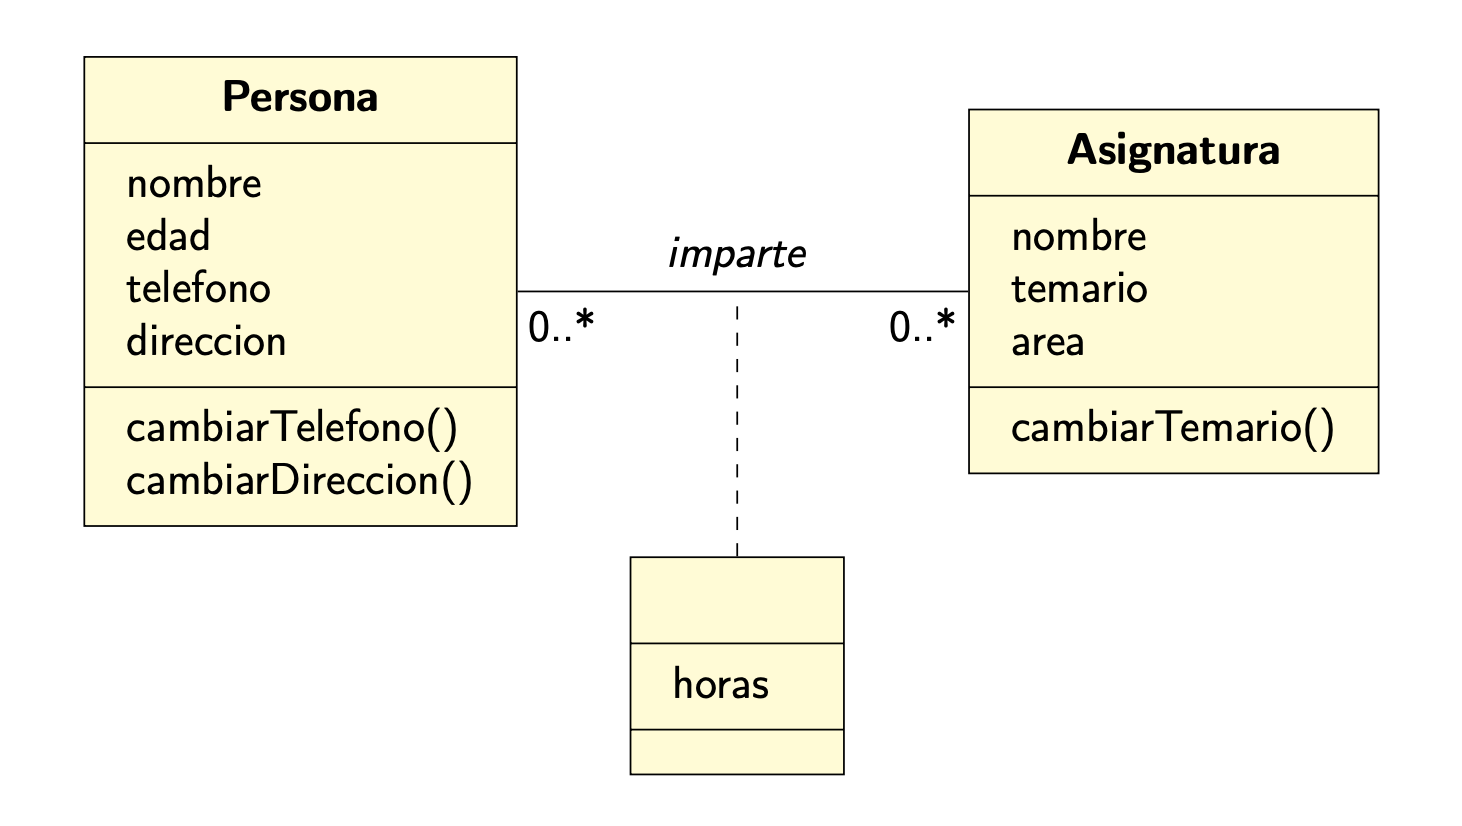
\includegraphics[width=\textwidth]{Imagenes/atribenlace.png}
	\caption{Asociación con atributo de enlace}
\end{figure}
\\
Vemos que una persona imparte asignaturas un número de horas y las asignaturas son impartidas por personas un número de horas.\vspace*{0.2cm}\\
Dependiendo de la multiplicidad podemos hacer que dicho atributo pertenezca a una de las dos clases (la que tiene mayor multiplicidad).\vspace*{0.2cm}
Si Asignatura tuviera multiplicidad 1, el atributos \textit{horas} iría en la clase Persona → hacemos uso de un conjunto ‘\texttt{set}’.\vspace*{0.2cm}\\
En este caso, ambos tienen multiplicidad muchos - muchos, por tanto, ese atributo no puede almacenarse en ninguna de las dos clases → tenemos que hacer uso de un diccionario ‘\texttt{map}’.
\newpage
\subsection{Implementación de la relación:}

\begin{lstlisting}[frame=single]
class Persona{
  public:
    typedef std::map<Asignatura*,tipo_atributo>Bs;
    void setA(Asignatura&, tipo_atributo);
    const Bs& getB()const;
  private:
    Bs bs_;
};

class Asignatura{
  public:
    typedef std::map<Persona*,tipo_atributo>As;
    void setB(Persona&, tipo_atributo);
    const As& getA()const;
  private:
    As as_;
};
\end{lstlisting}
